\documentclass[11pt]{article}

\usepackage{graphicx}
\usepackage{hyperref}

\graphicspath{{img/}}

\title{Path Planning}
\date{}

\begin{document}
\maketitle

\section{Introduction}
Path planning is the problem of finding a collision-free path for the robot from its starting configuration to a goal configuration. This is one of the oldest fundamental problems in robotics. Ideally, a path planning algorithm would guarantee to find a collision-free path whenever such a path exists.\\
Path planning is one of the most crucial research problems in robotics from the perspective of the control engineer. Many problems in various fields are solved by proposing path planning. It has been applied in guiding the robot to reach a particular objective from very simple trajectory planning to the selection of a suitable sequence of action. Path planning cannot always be designed in advance as the global environment information is not always available a priori. By proposing a proper algorithm, path planning can be widely applied in partially and unknown structured environments.
\section{Types of Path Planning Algorithms}
Multiple path planning and path finding
algorithms exist with varied applicability determined by the system’s kinematics, the
environment’s dynamics, robotic computation capabilities, and sensor- and other-sourced
information availability. Algorithm performance and complexity trade-offs also depend on
the use case.
An effective path planning algorithm needs to satisfy four criteria. First, the motion
planning technique must be capable of always finding the optimal path in realistic static
environments. Second, it must be expandable to dynamic environments. Third, it must
remain compatible with and enhance the chosen self-referencing approach. Fourth, it must
minimize the complexity, data storage, and computation time
\subsection{Dijkstra Algorithm}
The Dijkstra algorithm works by solving sub-problems computing the shortest path
from the source to vertices among the closest vertices to the source. It finds the next
closest vertex by maintaining the new vertices in a priority-min queue and stores only one
intermediate node so that only one shortest path can be found.
Dijkstra algorithm and its variants, which are commonly
used in applications, such as Google Maps and other traffic routing systems.

To overcome Dijkstra’s computational-intensity doing blind searches, \\ 
\textbf{A*} and its variants
are presented as state of the art algorithms for use within static environments.

\textbf{The Floyd algorithm} is a popular graph algorithm for finding the shortest path in
a positive or negative weighted graph, whereas Dijkstra works best for finding the single-source (finding shortest paths from a source vertex to all other vertices present in
the graph) shortest path in a positive weighted graph

\begin{figure}[h]
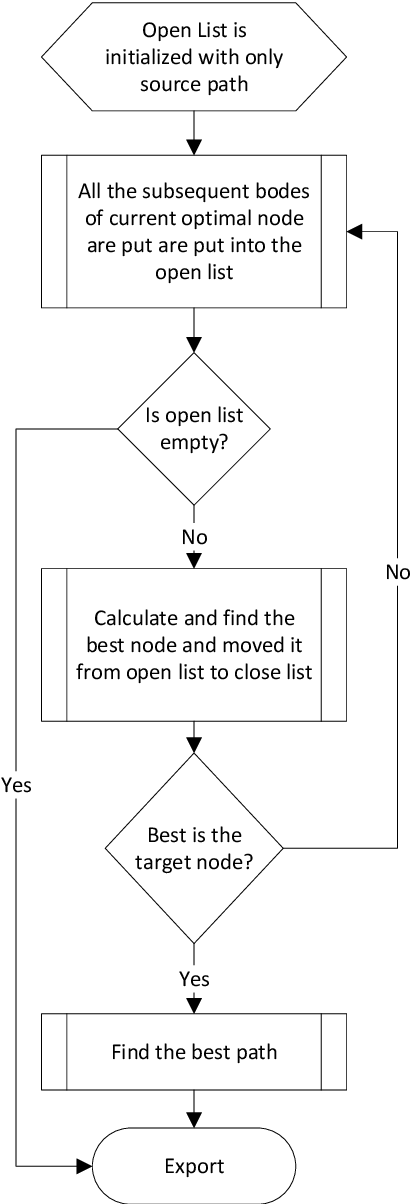
\includegraphics[width = 5cm,height = 8cm]{Dijkstra}
\caption{Flowchart of the improved Dijkstra algorithm used in path planning.}
\end{figure}


\subsection{A* Algorithm}

The A* Algorithm is a popular graph traversal path planning algorithm. A* operates
similarly to Dijkstra’s algorithm except that it guides its search towards the most promising
states, potentially saving a significant amount of computation time. A* is the most
widely used for approaching a near optimal solution with the available data-set/node.

It is widely used in static environments; there are instances where this algorithm
is used in dynamic environments. The base function can be tailored to a specific
application or environment based on our needs. A* is similar to Dijkstra in that it works
based on the lowest cost path tree from the initial point to the final target point. The base
algorithm uses the least expensive path and expands it using the function shown below$$f(n) = g(n) + h(n)$$
where g(n) is the actual cost from node n to the initial node, and h(n) is the cost of the
optimal path from the target node to n.

The A* algorithm is widely used in the gaming industry, and with the development of artificial intelligence, the A* algorithm has since been improved and tailored for
applications, including robot path planning, urban intelligent transportation, graph theory,
and automatic control.

\subsection{D* Algorithm}
Path planning in partially known and dynamic environments in an efficient manner
is increasingly critical, e.g., for automated vehicles. To solve this problem, the D* (or
Dynamic A*) algorithm is used to generate a collision-free path amidst moving obstacles.
D* is an informed incremental search algorithm that repairs the cost map partially and the
previously calculated cost map.

\subsection{Rapidly-Exploring Random Tree}
We have discussed algorithms like A*, which are static in nature and require a
path specified to them upfront. Let us now discuss dynamic and online algorithms like
\textbf{RRT}, which do not require a path to be specified upfront. Rather, they expand in all
regions, and, based on weights assigned to each node, create a path from start to goal. RRT’s
were introduced to handle broad classes of path planning problems. They were specifically
designed to handle non-holonomic constraints (constraints that are non-integrable into
positional constraints).
\begin{figure}[h]
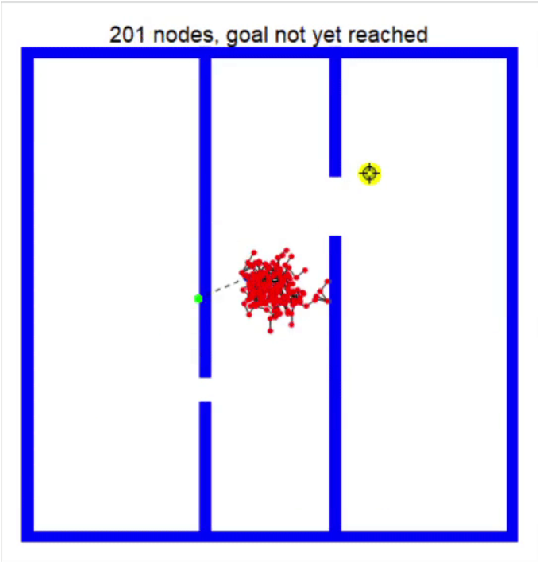
\includegraphics[width = 5cm,height = 5cm]{naive-random-tree}
\caption{Exploration of naive random tree selects a node at random from the tree and adds an edge
in a random direction.}
\end{figure}
\begin{figure}[h!]
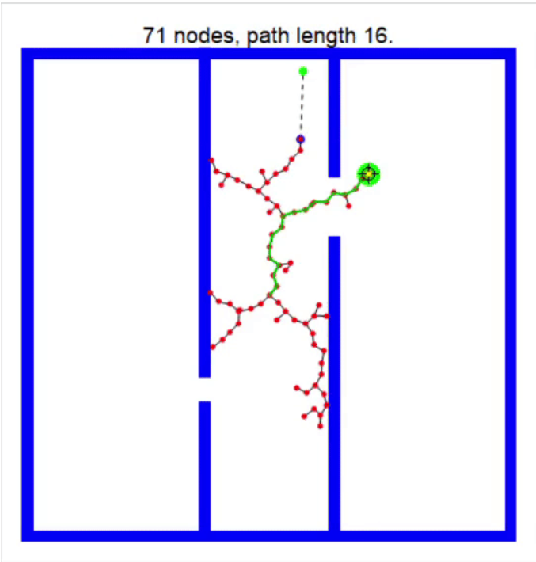
\includegraphics[width = 5cm,height = 5cm]{rapidly-exploring-random-tree}
\caption{rapidly-exploring random tree designed to explore paths in a high-dimensional space}
\end{figure}


RRT’s expand by rapidly sampling the space, grow from the starting point, and expand
until the tree is sufficiently close to goal point. In every iteration, the tree expands to the
nearest vertex of the randomly generated vertex. This nearest vertex is selected in terms of
a distance metric. It can be Euclidean, Manhattan, or any other distance metric.\pagebreak

\section{Global Planner and Local Planner}
The aim of solving this NP-hardness is not to find one solution that connects the start point and the goal point, but the optimal solution with the minimum distance and the smoothest maneuvers and without hitting any known obstacles. Usually, this module is divided into the global planner, which uses a priori information of the environment to create the best possible path, if any, and the local planner, which recalculates the initial plan to avoid possible dynamic obstacles.

\subsection{Global Planner}
As said before, the global planner requires a map of the environment to calculate the best route. Depending on the analysis of the map, some methods are based on Roadmaps like Silhouette proposed by Canny in 1987 or Voronoi in 2007. Some of them solve the problem by assigning a value to each region of the roadmap in order to find the path with minimum cost. Some examples are the \textbf{Dijkstra algorithm}, Best First, and \textbf{A*}. Another approach is by dividing the map into small regions (cells) called cell decomposition, the most extended algorithm used few years ago rapidly exploring random trees or the new approach based on neural networks. Some solutions combine the aforementioned algorithms improving the outcome at the cost of high computational power.
\subsection{Local Planner}
n order to transform the global path into suitable waypoints, the local planner creates new waypoints taking into consideration the dynamic obstacles and the vehicle constraints. So, to recalculate the path at a specific rate, the map is reduced to the surroundings of the vehicle and is updated as the vehicle is moving around. It is not possible to use the whole map because the sensors are unable to update the map in all regions and a large number of cells would raise the computational cost. Therefore, with the updated local map and the global waypoints, the local planning generates avoidance strategies for dynamic obstacles and tries to match the trajectory as much as possible to the provided waypoints from the global planner.

\section{Current Challenges}
Apart from current regulations that prohibit AV’ operation beyond the visual line of sight, safety concerns in instances of mechanical failure, and AV navigation in a GPS-denied environment, there are other limitations that need to be considered when developing a practical path planning algorithm. In this section, we go over four major limitations: the limited battery capacity of AV, onboard computational capabilities of AV, extreme weather conditions, and dynamic environments.

\subsection{Energy Constraints}
Although rotary-wing drones are highly maneuverable and versatile, they are still limited in terms of endurance. Thus, a single rotary-wing drone cannot be used for missions requiring long flight distances. Many factors can affect the battery performance of drones. Many maneuvers, such as hovering, horizontal and vertical movements, payload, speed, and flying in the wind direction, can impact drones’ battery performance at varying levels. In many studies, it is often assumed that drones can navigate through a computed path on a single charge. However, in practical settings, drones may often need to stop and recharge in order to navigate to their destination.
\subsection{Onboard Computational capabilities}
For many tasks, such as autonomous navigation, vision processing, localization of a drone, and mapping of the environment, the onboard computer requires high processing power and battery capacity. However, due to weight restrictions, onboard computers placed on drones have limited resources and onboard computational power.
\subsection{Dynamic Environment}
Collision avoidance in environments that are consistently changing has been a challenge for path planning for ground, underwater, and aerial vehicles. It is nearly impossible to obtain information about the entire environment prior to the takeoff of a drone. There can be stationary or moving objects that are placed after takeoff, which hinders the drone’s flight path. One area of research has been on developing better hardware to detect obstacles. There has been research focused on adding different types of sensors, such as LiDAR and ultrasonic sensors, to better detect obstacles during flight.
\section{Path Planning Future}
\textbf{Machine learning} methods are the latest development for determining robotic path planning. Reinforcement learning using Markov Decision Processes or deep neural networks can allow robots to modify their policy as it receives feedback on its environment. Classical Q-learning algorithms provide a model free learning environment.

\section{Practical Applications}
\begin{itemize}
\item\textbf{Autonomous vehicles}: Path planning algorithms enable self-driving cars to navigate through traffic and avoid collisions with other vehicles and pedestrians.
\item\textbf{Manufacturing logistics}: Robots in manufacturing facilities use path planning to move materials and products efficiently while avoiding collisions with other robots and obstacles.
\item\textbf{Planetary exploration}: Rovers on Mars or other planets use path planning algorithms to navigate through unknown terrain while avoiding hazards and minimizing energy consumption.
\end{itemize}

\section{Conclusion}
Recent years have seen the rapid growth of artificial intelligence in driverless vehicles
and other automated mobile systems. As a result, the amount of research into path planning
has increased dramatically. In the last decade, many new methods of path planning have
been developed; however, it is difficult to find a comprehensive survey on the most popular
path planning algorithms suitable for the novice practitioner

In this paper, we presented several widely used path planning algorithms and their
variants, categorized based primarily upon whether the environment in which the robot
operates is static or dynamic. In each section, we covered the methodology of all the
algorithms as well as their advantages and disadvantages, creating a comparative table
in each section for where each algorithm was suited best based on a static or dynamic
environment. The advances in computing and perception hardware have enabled us to use
complex algorithms for path planning.

We conclude that, for a given map the algorithm A* is a strong-performing option
for static environments because of the low memory usage, computational speed, less
implementation complexity, and efficiency making it suitable also for use in embedded
system deployment. One of the main limitations of bio-inspired algorithms is that they do
not have excellent results in real-time path planning as they have a possibility of becoming
stuck in local minima.

\section{References}
\begin{itemize}
\item Article,
\href{https://www.semanticscholar.org/paper/A-Survey-of-Path-Planning-Algorithms-for-Mobile-Karur-Sharma/9c07679d2da571ac6b9a051f229da4272817873d}{A Survey of Path Planning Algorithms for Mobile Robots}
\item Article,
\href{https://www.sciencedirect.com/science/article/abs/pii/B9780128202760000108}{Unmanned aerial systems: autonomy, cognition, and control}
\item \href{https://fab.cba.mit.edu/classes/865.21/topics/path_planning/robotic.html#:~:text=Machine%20learning%20methods%20are%20the%20latest%20development%20for,Q-learning%20algorithms%20provide%20a%20model%20free%20learning%20environment.}{Robotic Path planning}
\end{itemize}



\end{document}